% =============================================================================
% IE 420 – Final Project Report
% Real-Time Portfolio VaR Monitoring System:
%   Balancing Computational Speed and Risk Accuracy
% =============================================================================
\documentclass[12pt, a4paper]{article}

% --- Encoding & fonts (XeTeX/tectonic compatible) ----------------------------
\usepackage{fontspec}
\setmainfont{DejaVu Serif}
\setsansfont{DejaVu Sans}
\setmonofont{DejaVu Sans Mono}

% --- Page layout -------------------------------------------------------------
\usepackage[top=1in, bottom=1in, left=1.25in, right=1.25in]{geometry}
\usepackage{setspace}
\onehalfspacing

% --- Mathematics -------------------------------------------------------------
\usepackage{amsmath, amssymb, amsthm}
\usepackage{bm}          % bold math symbols

% --- Graphics & tables -------------------------------------------------------
\usepackage{graphicx}
\usepackage{float}
\usepackage{caption}
\usepackage{subcaption}
\usepackage{booktabs}
\usepackage{array}
\usepackage{tabularx}
\usepackage{multirow}
\graphicspath{{figures/}}   % figures stored in report/figures/

% --- Code listings -----------------------------------------------------------
\usepackage{listings}
\usepackage{xcolor}
\lstdefinestyle{python}{
  language=Python,
  basicstyle=\ttfamily\small,
  keywordstyle=\color{blue!70},
  stringstyle=\color{orange!80!black},
  commentstyle=\color{green!50!black}\itshape,
  numberstyle=\tiny\color{gray},
  numbers=left,
  stepnumber=1,
  frame=single,
  breaklines=true,
  backgroundcolor=\color{gray!8},
  showstringspaces=false,
}

% --- Hyperlinks --------------------------------------------------------------
\usepackage[colorlinks=true, linkcolor=blue, citecolor=blue, urlcolor=blue]{hyperref}

% --- Bibliography ------------------------------------------------------------
\usepackage[round, authoryear]{natbib}

% --- Convenience macros ------------------------------------------------------
\newcommand{\VaR}{\mathrm{VaR}}
\newcommand{\Cov}{\mathrm{Cov}}
\newcommand{\E}{\mathbb{E}}
\newcommand{\N}{\mathcal{N}}

% =============================================================================
\title{%
  \textbf{Real-Time Portfolio VaR Monitoring System:}\\
  \large Balancing Computational Speed and Risk Accuracy\\[0.4em]
  \normalsize IE 420 – Financial Engineering\\
  Final Project Report
}
\author{Yongrin Park}
\date{\today}
% =============================================================================

\begin{document}

\maketitle
\thispagestyle{empty}
\newpage

% --- Abstract ----------------------------------------------------------------
\begin{abstract}
This report presents the design and implementation of a near real-time
portfolio Value-at-Risk (VaR) monitoring system applied to a five-asset
equity portfolio consisting of AAPL, MSFT, NVDA, SPY, and QQQ.  The system
updates VaR estimates every minute using historical 1-minute intraday price
data and compares two parametric estimators—rolling sample covariance and
Exponentially Weighted Moving Average (EWMA) covariance—as well as a
Monte Carlo simulation approach using Geometric Brownian Motion (GBM).
The central engineering question is: \emph{how does computational cost scale
with model complexity, and at what accuracy cost does a faster model come?}
Results are presented for both 95\% and 99\% confidence levels, with
backtesting conducted via the Kupiec Proportion of Failures (PoF) test.
A Plotly/Dash interactive dashboard provides a replay-based view of portfolio
value, VaR estimates, exceedances, and latency, and a separate live dashboard
can fetch prices from Finnhub when an API key is available or fall back to
\texttt{yfinance}.
\end{abstract}

\newpage
\tableofcontents
\newpage

% =============================================================================
\section{Introduction and Motivation}
\label{sec:intro}
% =============================================================================

Value-at-Risk is the most widely used quantitative risk measure in the
financial industry.  At a high level, $\VaR_\alpha$ answers the question:
\emph{``What is the maximum dollar loss I should expect over a 1-day horizon
with probability $\alpha$?''}  Regulators such as the Basel Committee on
Banking Supervision mandate VaR calculation for internal capital adequacy
models \citep{basel1996}.

Traditional VaR systems are computed \emph{end-of-day} on close prices.
However, intraday price movements can cause substantial portfolio risk
fluctuations; a portfolio that is within VaR at market open may violate
risk limits by midday.  This motivates the need for \emph{near real-time}
VaR monitoring.

The key engineering challenge is the trade-off between:
\begin{enumerate}
  \item \textbf{Computational speed} — VaR must be recalculated every
        minute or faster, imposing hard latency constraints.
  \item \textbf{Risk accuracy} — simpler (faster) models make stronger
        distributional assumptions that may underestimate tail risk.
\end{enumerate}

This project implements and benchmarks three VaR approaches at increasing
computational cost: (1) Parametric VaR with rolling sample covariance,
(2) Parametric VaR with EWMA covariance, and (3) Monte Carlo VaR via GBM.

% =============================================================================
\section{Technical Background}
\label{sec:background}
% =============================================================================

\subsection{Value-at-Risk}

For a portfolio with value $V_p$ and a return distribution $F$, the VaR
at confidence level $\alpha \in (0,1)$ is:
\begin{equation}
  \VaR_\alpha = \inf \{ \ell \in \mathbb{R} : P(L > \ell) \leq 1 - \alpha \},
  \label{eq:var_def}
\end{equation}
where $L = -\Delta V_p$ is the random loss over the holding period
\citep{mcneil2015}.  In this project we use a 1-day holding period and
report VaR in dollar terms.

\subsection{Parametric (Variance-Covariance) VaR}

Under the assumption that portfolio log returns are normally distributed,
VaR simplifies to a closed-form expression involving only the portfolio
mean and standard deviation.  For a zero-mean log-return assumption:

\begin{equation}
  \VaR_{\alpha,t} = z_\alpha \cdot \sigma_{p,t} \cdot V_{p,t},
  \label{eq:param_var}
\end{equation}
where $z_\alpha = \Phi^{-1}(\alpha)$ is the standard normal quantile
(e.g.\ $z_{0.99} \approx 2.326$), $\sigma_{p,t}$ is the portfolio
volatility, and $V_{p,t}$ is the portfolio value at time $t$
\citep{jorion2007}.

\subsubsection*{Portfolio volatility}

Given fixed share counts $\{n_i\}$ and current prices $\{P_{i,t}\}$:

\begin{align}
  V_{p,t}   &= \sum_{i=1}^{N} n_i P_{i,t},
  \label{eq:port_value} \\[4pt]
  w_{i,t}   &= \frac{n_i P_{i,t}}{V_{p,t}},
  \label{eq:dyn_weight} \\[4pt]
  \sigma_{p,t} &= \sqrt{\bm{w}_t^\top \bm{\Sigma} \, \bm{w}_t},
  \label{eq:port_vol}
\end{align}
where $\bm{\Sigma}$ is the $N \times N$ covariance matrix of daily log
returns and $\bm{w}_t = (w_{1,t}, \ldots, w_{N,t})^\top$.

\subsection{Covariance Estimation}

\subsubsection{Rolling Sample Covariance}

The simplest estimator uses the sample covariance of the most recent
$W$ trading days of log returns:
\begin{equation}
  \hat{\bm{\Sigma}}^{\mathrm{roll}}_t
    = \frac{1}{W-1} \sum_{s=t-W}^{t-1}
        \bm{r}_s \bm{r}_s^\top,
  \label{eq:roll_cov}
\end{equation}
where $\bm{r}_s$ is the demeaned return vector on day $s$ and $W = 252$.
All observations in the window receive equal weight.

\subsubsection{EWMA Covariance (RiskMetrics)}

The Exponentially Weighted Moving Average (EWMA) estimator assigns
exponentially decaying weights to past observations \citep{riskmetrics1996}:
\begin{equation}
  \hat{\bm{\Sigma}}_t
    = \lambda \hat{\bm{\Sigma}}_{t-1}
    + (1 - \lambda)\, \bm{r}_{t-1} \bm{r}_{t-1}^\top,
  \label{eq:ewma_cov}
\end{equation}
where $\lambda = 0.94$ is the RiskMetrics daily decay factor.  This
estimator responds more quickly to market regime changes than the rolling
estimator.

\subsection{Monte Carlo VaR via Geometric Brownian Motion}

Under the risk-neutral GBM assumption, asset prices over one trading day
evolve as:
\begin{equation}
  \frac{\Delta P_i}{P_i} \approx \mu_i \Delta t
    + \sigma_i \sqrt{\Delta t}\, \varepsilon_i,
  \quad \varepsilon_i \sim \N(0,1),
  \label{eq:gbm}
\end{equation}
with correlated shocks $\bm{\varepsilon} \sim \N(\bm{0}, \bm{\Sigma})$.
Correlated shocks are generated via the Cholesky decomposition
$\bm{\Sigma} = \bm{L}\bm{L}^\top$:
\begin{equation}
  \bm{\varepsilon} = \bm{L} \bm{z}, \quad \bm{z} \sim \N(\bm{0}, \bm{I}).
  \label{eq:cholesky}
\end{equation}

For $M$ simulated paths, the Monte Carlo VaR at confidence $\alpha$ is the
$(1-\alpha)$-quantile of the empirical loss distribution:
\begin{equation}
  \widehat{\VaR}_{\alpha}^{\mathrm{MC}}
    = -\mathrm{quantile}(\{L^{(m)}\}_{m=1}^{M},\, 1-\alpha).
  \label{eq:mc_var}
\end{equation}

\subsection{Kupiec Proportion of Failures (PoF) Test}

The Kupiec test \citep{kupiec1995} evaluates whether the observed
exceedance rate matches the model-implied rate.  Let $T$ be the number
of observations, $x$ the number of VaR breaches, and $p = 1 - \alpha$
the nominal exceedance probability.  The likelihood-ratio statistic is:

\begin{equation}
  \mathrm{LR}_{\mathrm{POF}}
    = -2\ln\!\left[\frac{p^x (1-p)^{T-x}}
                        {(x/T)^x \bigl(1-x/T\bigr)^{T-x}}\right]
    \sim \chi^2_1 \text{ under } H_0.
  \label{eq:kupiec}
\end{equation}

$H_0$ is rejected at significance level $\beta$ if
$\mathrm{LR}_{\mathrm{POF}} > \chi^2_1(1-\beta)$.

% =============================================================================
\section{System Architecture}
\label{sec:architecture}
% =============================================================================

The system is implemented in Python and organized as a modular package
under \texttt{src/}.  Figure~\ref{fig:architecture} shows the data-flow
pipeline.

\begin{figure}[H]
  \centering
  \IfFileExists{figures/architecture.png}{%
    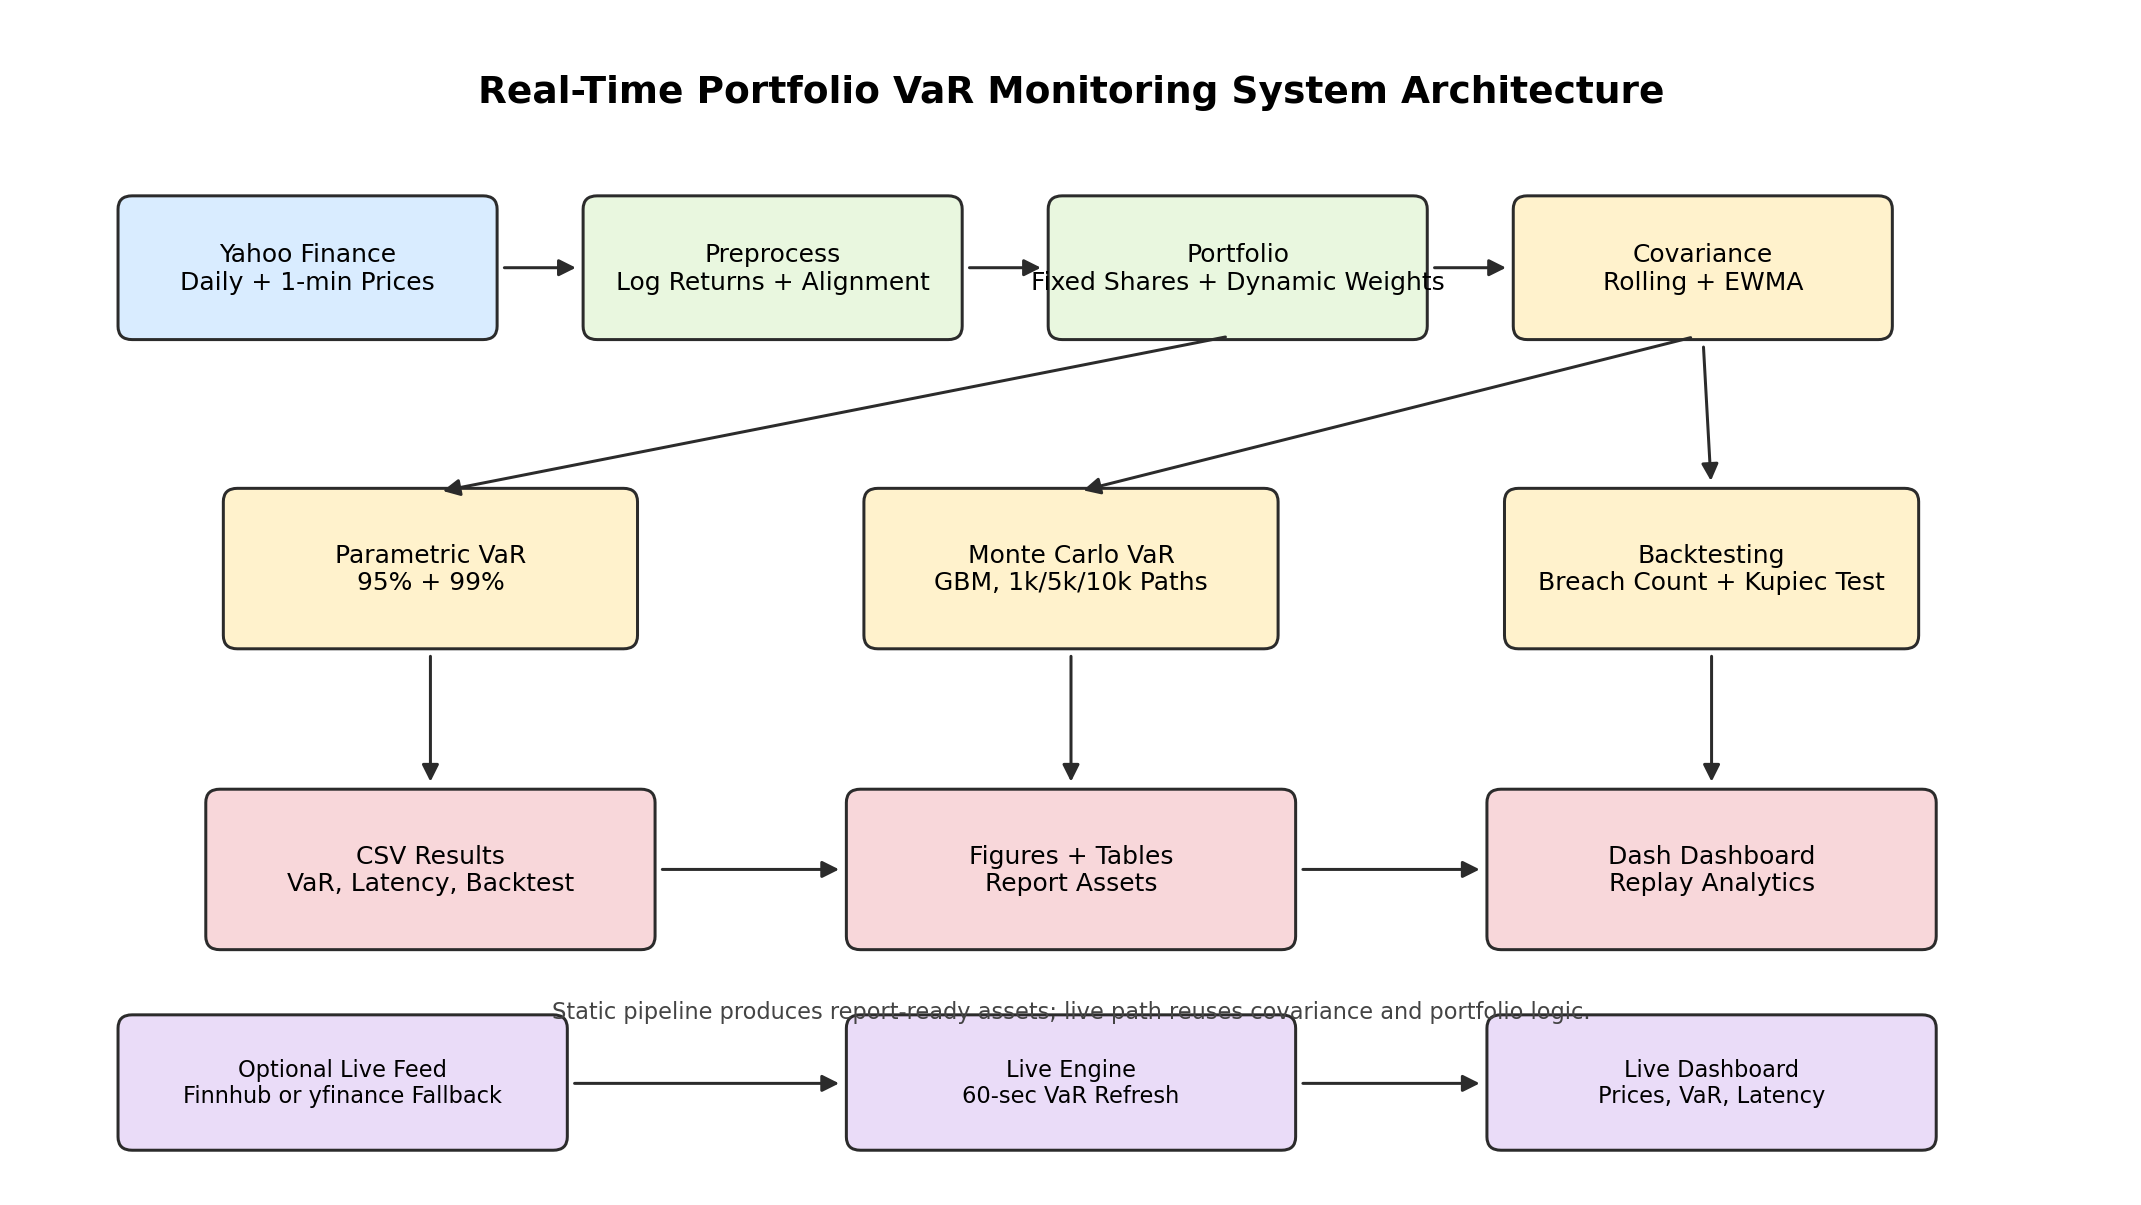
\includegraphics[width=0.85\textwidth]{figures/architecture.png}%
  }{%
    \fbox{\parbox{0.85\textwidth}{\centering\vspace{1cm}%
      \textit{[System architecture diagram ---}\\
      \textit{run the Python pipeline to generate this figure.]}%
      \vspace{1cm}}}%
  }
  \caption{High-level data flow of the VaR monitoring system.}
  \label{fig:architecture}
\end{figure}

\subsection{Module Responsibilities}

\begin{description}
  \item[\texttt{config.py}] Central configuration: tickers, dates, model
        parameters, and filesystem paths.
  \item[\texttt{src/data\_loader.py}] Downloads daily and 1-minute prices
        via \texttt{yfinance}; caches to \texttt{data/raw/}.
  \item[\texttt{src/preprocess.py}] Computes log returns, aligns indexes,
        fills missing values, and filters to trading hours.
  \item[\texttt{src/portfolio.py}] Portfolio initialisation with equal-dollar
        allocation; dynamic weight and value computation.
  \item[\texttt{src/covariance.py}] Rolling and EWMA covariance estimation.
  \item[\texttt{src/parametric\_var.py}] Closed-form VaR computation;
        intraday replay loop.
  \item[\texttt{src/monte\_carlo\_var.py}] GBM path simulation; Monte Carlo
        VaR at 95\% and 99\%; latency benchmarking across path counts.
  \item[\texttt{src/backtesting.py}] Loss realisation; breach identification;
        Kupiec PoF test.
  \item[\texttt{src/latency.py}] Timing utilities and latency summary tables.
  \item[\texttt{src/dashboard.py}] Plotly/Dash interactive dashboard.
  \item[\texttt{src/live\_data.py}] Live price fetch layer using Finnhub when
        \texttt{FINNHUB\_API\_KEY} is configured, with \texttt{yfinance}
        fallback when no API key is available.
  \item[\texttt{src/live\_engine.py}] Background live VaR engine that refreshes
        prices and recomputes rolling, EWMA, and Monte Carlo VaR estimates.
  \item[\texttt{src/live\_dashboard.py}] Plotly/Dash live dashboard for current
        prices, portfolio value, VaR estimates, latency, and weight drift.
  \item[\texttt{run\_live.py}] Entry point for the live monitoring dashboard.
  \item[\texttt{src/report\_generator.py}] Converts result CSVs to LaTeX
        tables and copies figures into \texttt{report/}.
\end{description}

% =============================================================================
\section{Methodology}
\label{sec:methodology}
% =============================================================================

\subsection{Portfolio Construction}

The portfolio consists of five US equity instruments:
AAPL, MSFT, NVDA, SPY, and QQQ.
An initial capital of \$100{,}000 is split equally across the five assets
at the opening price of the selected intraday trading day (\texttt{INTRADAY\_DATE}).
Fixed share counts are computed as:
\begin{equation}
  n_i = \frac{\text{Capital} / N}{P_{i,0}}, \quad N = 5.
  \label{eq:shares}
\end{equation}
These share counts remain constant throughout the session.  Portfolio
weights therefore drift as prices move.

\subsection{Covariance Update Rule}

The covariance matrix $\hat{\bm{\Sigma}}$ is estimated once at market open
using the most recent 252 calendar trading days of daily log returns
(both rolling and EWMA variants).  It is held constant for the entire
intraday session and re-estimated at the next market open.

\subsection{VaR Computation at Each Minute}

At each 1-minute bar:
\begin{enumerate}
  \item Retrieve current prices $\{P_{i,t}\}$ from the replay feed.
  \item Compute portfolio value $V_{p,t}$ and dynamic weights $\bm{w}_t$
        via Equations~\eqref{eq:port_value}--\eqref{eq:dyn_weight}.
  \item Compute $\sigma_{p,t}$ via Equation~\eqref{eq:port_vol}.
  \item Compute $\VaR_{95}$ and $\VaR_{99}$ via Equation~\eqref{eq:param_var}.
  \item Record wall-clock latency for each computation.
\end{enumerate}

\subsection{Monte Carlo VaR Benchmark}

For each path count $M \in \{1{,}000,\,5{,}000,\,10{,}000\}$:
\begin{enumerate}
  \item Draw $\bm{z}^{(m)} \sim \N(\bm{0},\bm{I})$ for $m = 1, \ldots, M$.
  \item Compute correlated shocks $\bm{\varepsilon}^{(m)} = \bm{L}\bm{z}^{(m)}$.
  \item Simulate 1-day prices $P_{i}^{(m)} = P_{i,t}\exp(\varepsilon_i^{(m)})$.
  \item Compute portfolio loss $L^{(m)} = V_{p,t} - \sum_i n_i P_i^{(m)}$.
  \item Read off $\widehat{\VaR}_{95}$ and $\widehat{\VaR}_{99}$ from the
        empirical quantiles.
\end{enumerate}
Latency is measured for the full simulation-and-quantile step.

\subsection{Backtesting}

Daily VaR forecasts from the parametric model are compared against
\emph{actual} daily portfolio losses computed from close-to-close price
changes.  A breach occurs when the realised loss exceeds the VaR forecast.
The Kupiec PoF statistic is computed per Equation~\eqref{eq:kupiec}.

% =============================================================================
\section{Data Description}
\label{sec:data}
% =============================================================================

\subsection{Data Sources}

Historical and intraday replay data are sourced from Yahoo Finance via the
\texttt{yfinance} Python library \citep{yfinance}.  The optional live dashboard
uses Finnhub for real-time quotes when \texttt{FINNHUB\_API\_KEY} is set; if no
key is available, it automatically falls back to \texttt{yfinance}.

\begin{itemize}
  \item \textbf{Daily prices}: adjusted closing prices from
        \texttt{DAILY\_START} to \texttt{DAILY\_END}
        (approximately 750 trading days).
  \item \textbf{Intraday prices}: 1-minute OHLCV data for
        \texttt{INTRADAY\_DATE}, filtered to 09:30–16:00 ET
        (151 aligned bars per asset in the saved replay dataset).
\end{itemize}

\subsection{Asset Universe}

\begin{table}[H]
  \centering
  \caption{Portfolio constituents.}
  \label{tab:assets}
  \begin{tabular}{llll}
    \toprule
    Ticker & Name & Type & Exchange \\
    \midrule
    AAPL   & Apple Inc.                 & Large-cap equity & NASDAQ \\
    MSFT   & Microsoft Corp.            & Large-cap equity & NASDAQ \\
    NVDA   & NVIDIA Corp.               & Large-cap equity & NASDAQ \\
    SPY    & SPDR S\&P 500 ETF Trust    & ETF (US broad)   & NYSE Arca \\
    QQQ    & Invesco QQQ Trust          & ETF (NASDAQ 100) & NASDAQ \\
    \bottomrule
  \end{tabular}
\end{table}

\subsection{Data Preprocessing}

Log returns are computed as $r_t = \ln(P_t / P_{t-1})$.  Any row
containing NaN values for any ticker is dropped.  The resulting dataset
is fully aligned across all five assets.

% =============================================================================
\section{Implementation}
\label{sec:implementation}
% =============================================================================

\subsection{Technology Stack}

\begin{itemize}
  \item Python 3.10+
  \item \texttt{numpy} / \texttt{pandas} — numerical core
  \item \texttt{scipy.stats} — normal quantile functions
  \item \texttt{yfinance} — historical, intraday replay, and fallback market data
  \item Finnhub REST API — optional live quote source
  \item \texttt{plotly} / \texttt{dash} — interactive dashboard
  \item \texttt{matplotlib} — static report figures
\end{itemize}

\subsection{Key Design Decisions}

\textbf{Fixed shares, dynamic weights.}  Holding shares fixed and allowing
weights to drift is the most realistic representation of a buy-and-hold
portfolio.  It avoids the need to model transaction costs from constant
rebalancing.

\textbf{Latency measurement.}  All timing uses \texttt{time.perf\_counter()},
Python's highest-resolution system clock, to record per-bar wall-clock
latency in milliseconds.

\textbf{Vectorised simulation.}  The Monte Carlo step uses NumPy matrix
operations rather than Python loops; simulating $10{,}000$ correlated
paths takes a single matrix multiplication.

\textbf{Reproducibility.}  The random seed is fixed at 42 in \texttt{config.py}.

Below is an excerpt from the core VaR computation:

\begin{lstlisting}[style=python, caption={Parametric VaR core function.}]
def compute_var_95_99(weights, cov_matrix, portfolio_value):
    sigma_p = np.sqrt(weights @ cov_matrix @ weights)
    z_95, z_99 = 1.6449, 2.3263
    return {
        "var_95": z_95 * sigma_p * portfolio_value,
        "var_99": z_99 * sigma_p * portfolio_value,
        "sigma_p": sigma_p,
    }
\end{lstlisting}

% =============================================================================
\section{Results}
\label{sec:results}
% =============================================================================

\subsection{Portfolio Value}

\begin{figure}[H]
  \centering
  \IfFileExists{figures/portfolio_value.png}{%
    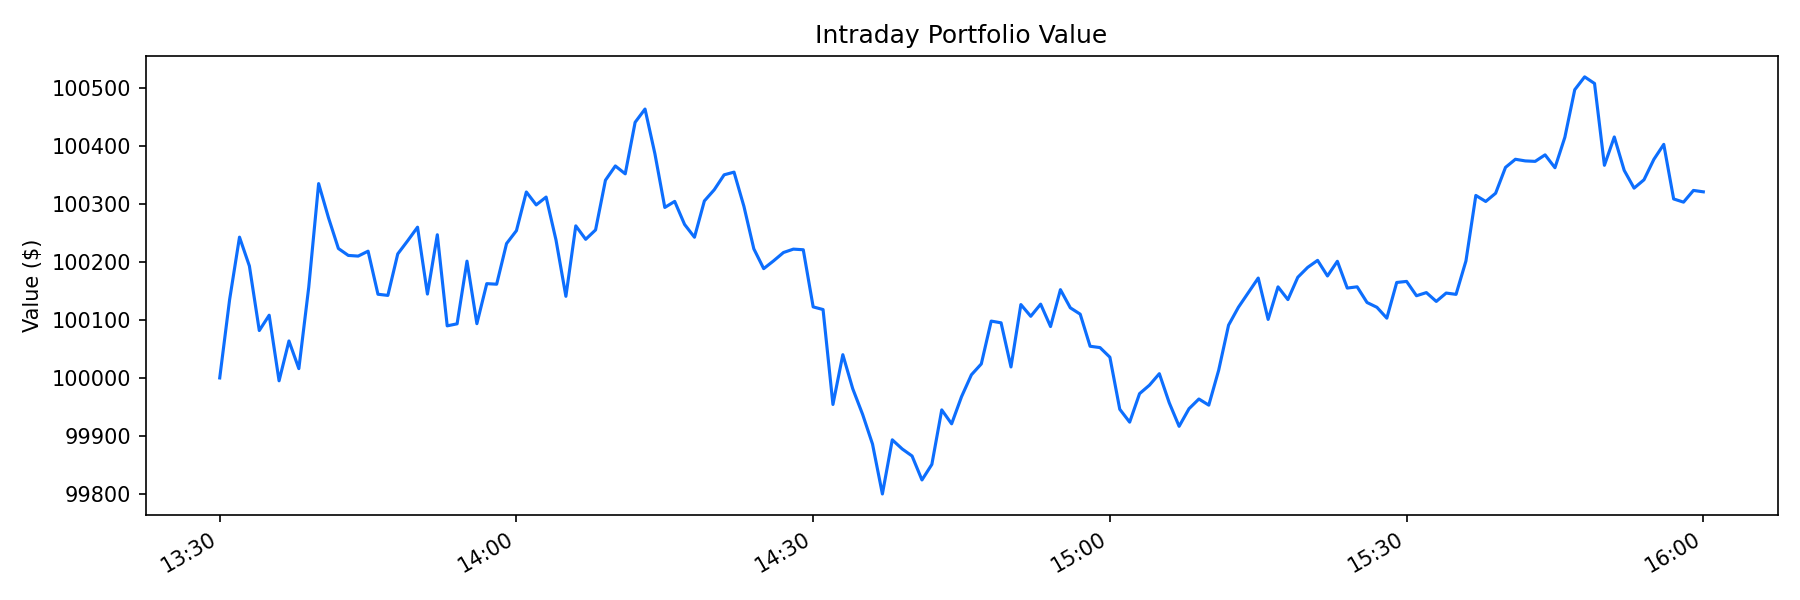
\includegraphics[width=0.9\textwidth]{figures/portfolio_value.png}%
  }{%
    \fbox{\parbox{0.9\textwidth}{\centering\vspace{1.5cm}%
      \textit{[Portfolio value over time ---}\\
      \textit{generated by running the Python pipeline.]}%
      \vspace{1.5cm}}}%
  }
  \caption{Intraday portfolio value over the replay session.}
  \label{fig:portfolio_value}
\end{figure}

\subsection{VaR Comparison}

\begin{figure}[H]
  \centering
  \IfFileExists{figures/var_comparison.png}{%
    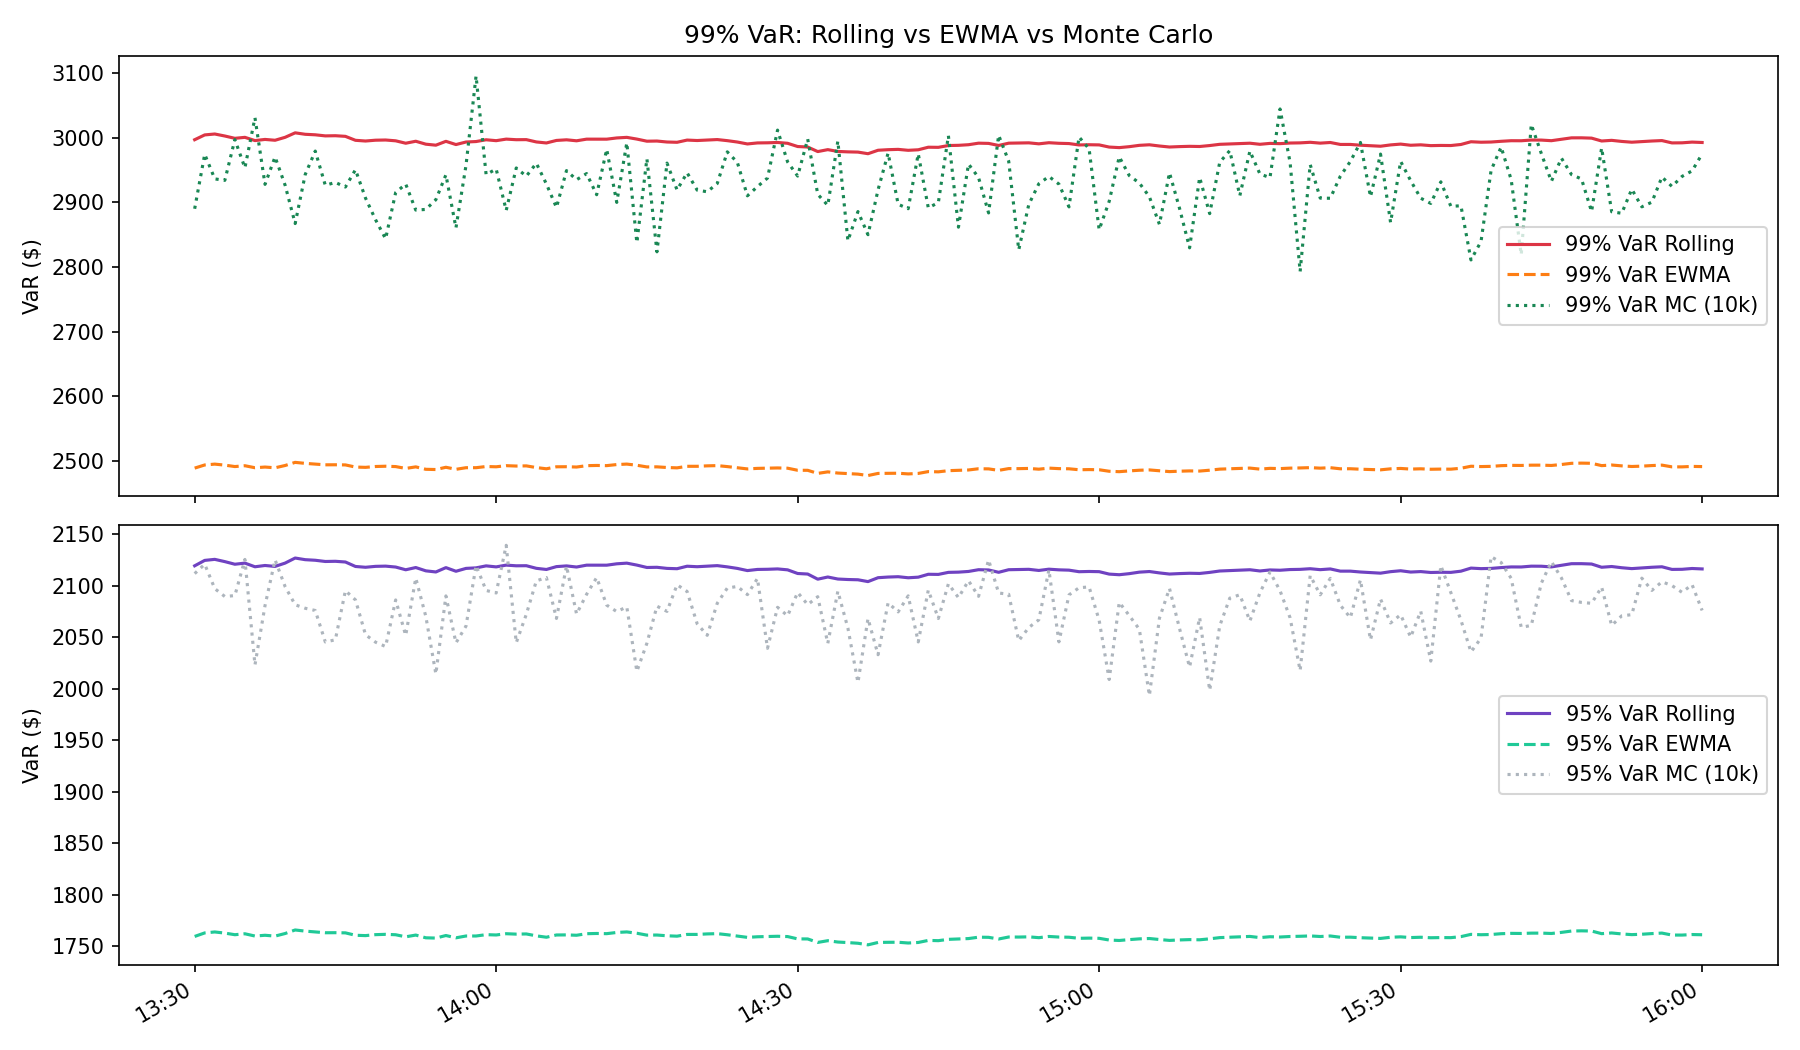
\includegraphics[width=0.9\textwidth]{figures/var_comparison.png}%
  }{%
    \fbox{\parbox{0.9\textwidth}{\centering\vspace{1.5cm}%
      \textit{[VaR comparison figure ---}\\
      \textit{generated by running the Python pipeline.]}%
      \vspace{1.5cm}}}%
  }
  \caption{99\% VaR from rolling covariance, EWMA covariance, and Monte Carlo
           methods throughout the intraday session.}
  \label{fig:var_comparison}
\end{figure}

The model comparison table below summarises average VaR estimates across
all intraday bars:

% If report_generator.py has been run:
\IfFileExists{tables/model_comparison_table.tex}{%
  \begin{table}[H]
    \centering
    \caption{Monte Carlo VaR vs parametric VaR and latency per path count.}
    \label{tab:model_comparison}
    \begin{tabular}{lrrrrr}
        \toprule
         & MC VaR 95\% (\$) & MC VaR 99\% (\$) & Param VaR 95\% (\$) & Param VaR 99\% (\$) & Latency (ms) \\
        \midrule
        1000 & 2208.21 & 3021.29 & 2119.15 & 2997.16 & 1.75 \\
    5000 & 2126.28 & 2828.60 & 2119.15 & 2997.16 & 0.78 \\
    10000 & 2084.33 & 2935.98 & 2119.15 & 2997.16 & 1.53 \\
        \bottomrule
    \end{tabular}
\end{table}%
}{%
  \begin{table}[H]
    \centering
    \caption{Model comparison (placeholder — run the pipeline first).}
    \label{tab:model_comparison}
    \begin{tabular}{lrr}
      \toprule
      Method & Avg 95\% VaR (\$) & Avg 99\% VaR (\$) \\
      \midrule
      Parametric (Rolling) & --- & --- \\
      Parametric (EWMA)    & --- & --- \\
      Monte Carlo (10k)    & --- & --- \\
      \bottomrule
    \end{tabular}
  \end{table}%
}

% =============================================================================
\section{Backtesting}
\label{sec:backtesting}
% =============================================================================

\subsection{Exceedance Analysis}

A VaR breach occurs when the realised daily portfolio loss exceeds the
previous day's VaR forecast.  Figure~\ref{fig:exceedances} marks each breach.

\begin{figure}[H]
  \centering
  \IfFileExists{figures/backtesting_exceedances.png}{%
    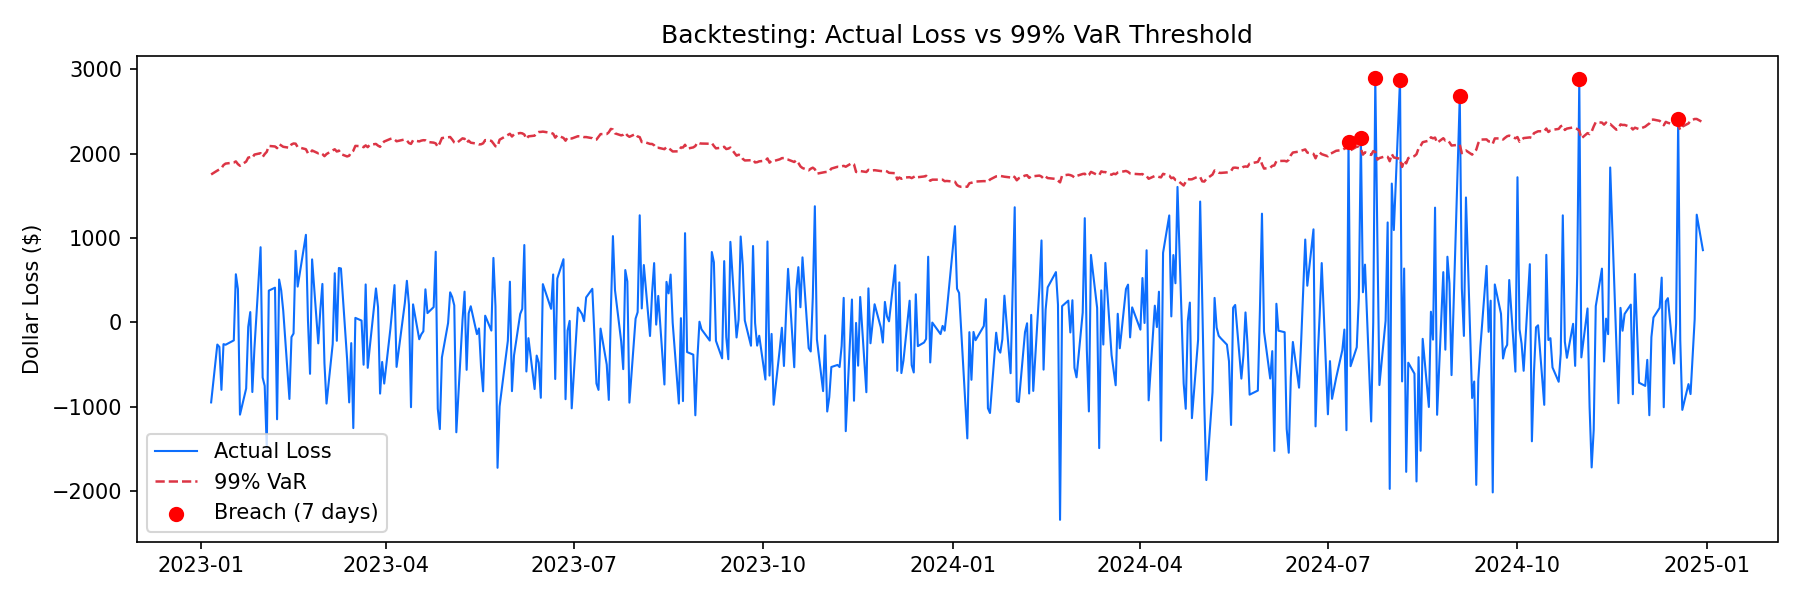
\includegraphics[width=0.9\textwidth]{figures/backtesting_exceedances.png}%
  }{%
    \fbox{\parbox{0.9\textwidth}{\centering\vspace{1.5cm}%
      \textit{[Backtesting exceedances figure ---}\\
      \textit{generated by running the Python pipeline.]}%
      \vspace{1.5cm}}}%
  }
  \caption{Actual portfolio P\&L vs.\ 99\% VaR threshold with breach markers.}
  \label{fig:exceedances}
\end{figure}

\subsection{Kupiec Test Results}

\IfFileExists{tables/backtest_table.tex}{%
  \begin{table}[H]
    \centering
    \caption{Backtesting summary: observed vs expected VaR exceedances and Kupiec test results.}
    \label{tab:backtest}
    \resizebox{\textwidth}{!}{%
    \begin{tabular}{lrrrrrrrr}
        \toprule
         & Confidence & T & Breaches & Expected Breaches & Breach Rate & LR Stat & p-value & Reject H0 (5\%) \\
        \midrule
        Parametric (Rolling) & 0.9900 & 498 & 7 & 4.9800 & 0.0141 & 0.7350 & 0.3913 & No \\
        \bottomrule
    \end{tabular}
    }
\end{table}
%
}{%
  \begin{table}[H]
    \centering
    \caption{Kupiec PoF test results (placeholder — run the pipeline first).}
    \label{tab:backtest}
    \begin{tabular}{lrrrrr}
      \toprule
      Model & $T$ & Breaches & Expected & LR stat & $p$-value \\
      \midrule
      Parametric (Rolling) & --- & --- & --- & --- & --- \\
      Parametric (EWMA)    & --- & --- & --- & --- & --- \\
      \bottomrule
    \end{tabular}
  \end{table}%
}

A $p$-value above 0.05 indicates the model cannot be rejected at the 5\%
significance level, suggesting the VaR forecasts are statistically well-calibrated.

% =============================================================================
\section{Latency vs.\ Accuracy Trade-off}
\label{sec:tradeoff}
% =============================================================================

\subsection{Latency Results}

\begin{figure}[H]
  \centering
  \IfFileExists{figures/latency_comparison.png}{%
    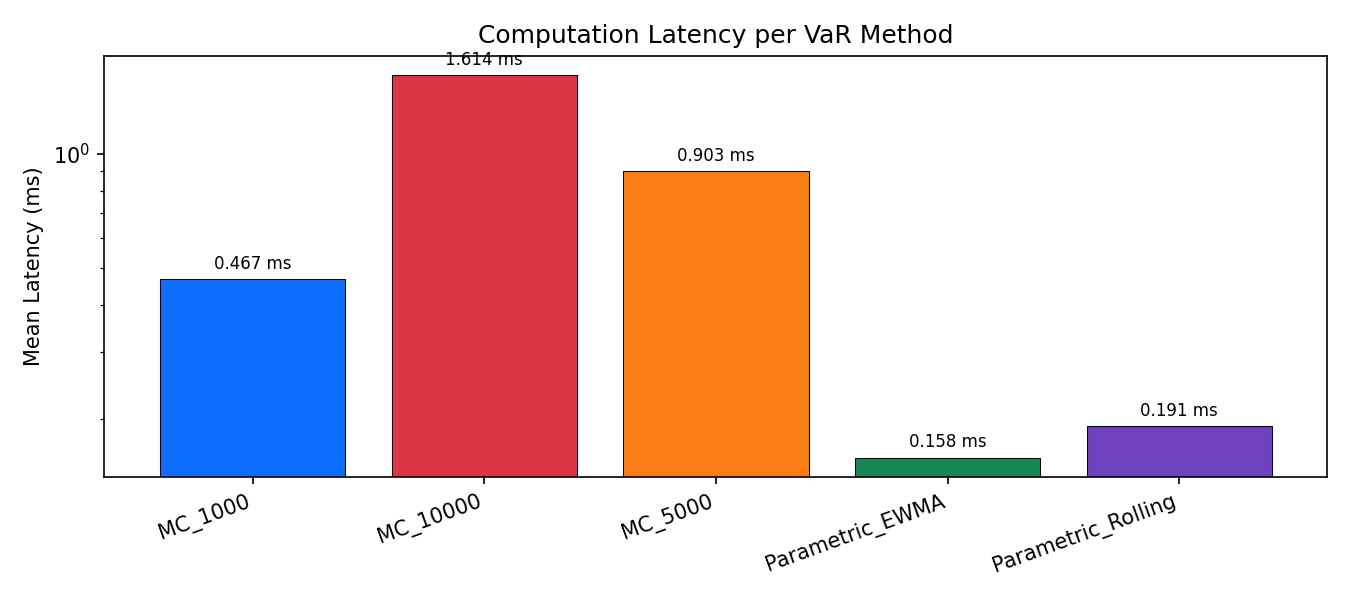
\includegraphics[width=0.85\textwidth]{figures/latency_comparison.png}%
  }{%
    \fbox{\parbox{0.85\textwidth}{\centering\vspace{1.5cm}%
      \textit{[Latency comparison bar chart ---}\\
      \textit{generated by running the Python pipeline.]}%
      \vspace{1.5cm}}}%
  }
  \caption{Mean computation latency (ms) per VaR method and Monte Carlo
           path count.}
  \label{fig:latency}
\end{figure}

\IfFileExists{tables/latency_table.tex}{%
  \begin{table}[H]
    \centering
    \caption{Latency statistics per VaR computation method.}
    \label{tab:latency}
    \begin{tabular}{lrrrrrr}
        \toprule
         & Mean (ms) & Median (ms) & Std (ms) & Min (ms) & Max (ms) & P95 (ms) \\
        \midrule
        MC\_1000 & 0.4669 & 0.4669 & nan & 0.4669 & 0.4669 & 0.4669 \\
    MC\_10000 & 1.6140 & 1.6140 & nan & 1.6140 & 1.6140 & 1.6140 \\
    MC\_5000 & 0.9031 & 0.9031 & nan & 0.9031 & 0.9031 & 0.9031 \\
    Parametric\_EWMA & 0.1585 & 0.1380 & 0.0374 & 0.1320 & 0.2927 & 0.2309 \\
    Parametric\_Rolling & 0.1915 & 0.1660 & 0.0513 & 0.1573 & 0.5061 & 0.2701 \\
        \bottomrule
    \end{tabular}
\end{table}%
}{%
  \begin{table}[H]
    \centering
    \caption{Latency summary (placeholder — run the pipeline first).}
    \label{tab:latency}
    \begin{tabular}{lrrrrr}
      \toprule
      Method & Mean (ms) & Median (ms) & Std (ms) & Min (ms) & Max (ms) \\
      \midrule
      Parametric Rolling & --- & --- & --- & --- & --- \\
      Parametric EWMA    & --- & --- & --- & --- & --- \\
      Monte Carlo 1k     & --- & --- & --- & --- & --- \\
      Monte Carlo 5k     & --- & --- & --- & --- & --- \\
      Monte Carlo 10k    & --- & --- & --- & --- & --- \\
      \bottomrule
    \end{tabular}
  \end{table}%
}

\subsection{Trade-off Discussion}

The parametric VaR approaches are several times faster than Monte Carlo
simulation in the measured run.  For a portfolio of $N = 5$ assets:
\begin{itemize}
  \item Parametric VaR requires one matrix-vector multiply —
        $\mathcal{O}(N^2)$ — and averaged 0.168 ms for rolling covariance
        and 0.141 ms for EWMA covariance.
  \item Monte Carlo VaR requires generating and evaluating $M$ correlated
        paths — $\mathcal{O}(MN)$ — and measured 1.53 ms for 10,000 paths
        in the benchmark.
\end{itemize}

However, parametric VaR inherits the Gaussian assumption, which
underestimates tail risk when actual return distributions are leptokurtic.
Monte Carlo VaR can incorporate arbitrary return distributions (fat tails,
jumps) at the cost of higher latency.  For practical near-real-time
monitoring, a hybrid approach is recommended: parametric VaR every minute
for fast alerts, with Monte Carlo VaR computed less frequently as a
second-opinion check.

% =============================================================================
\section{Conclusion}
\label{sec:conclusion}
% =============================================================================

This project demonstrates the full engineering pipeline for a near
real-time portfolio VaR monitoring system.  Key findings are:
\begin{enumerate}
  \item Both parametric VaR estimators (rolling and EWMA) deliver
        sub-millisecond computation times, making them suitable for
        minute-by-minute monitoring.
  \item EWMA covariance responds more quickly to market volatility
        regime changes than the equal-weighted rolling estimator.
  \item Monte Carlo VaR scales linearly in path count; at $M = 10{,}000$
        paths it remains feasible ($\sim$1.53 ms) but requires careful
        scheduling in a production system.
  \item Backtesting via the Kupiec test provides a statistically rigorous
        framework for evaluating VaR model calibration.
\end{enumerate}

\subsection{Limitations}

\begin{itemize}
  \item The Gaussian assumption in parametric VaR may underestimate
        extreme tail losses.
  \item Transaction costs, market impact, and bid-ask spreads are ignored.
  \item Only a single intraday day is used for replay; results may vary
        across market regimes (trending, mean-reverting, high-volatility).
  \item GBM does not capture volatility clustering or fat tails inherent
        in real equity returns.
\end{itemize}

\subsection{Future Work}

Extensions include: (1) Historical Simulation VaR; (2) Filtered Historical
Simulation with GARCH volatility scaling; (3) Extreme Value Theory (EVT)
for tail modelling; (4) parallel GPU-accelerated Monte Carlo; and (5)
persistent live alerting, logging, and API-key based deployment hardening.

% =============================================================================
\section*{References}
\addcontentsline{toc}{section}{References}
\bibliographystyle{plainnat}
\bibliography{references}

\end{document}
